\documentclass[a4paper,12pt]{report}
\usepackage[T2A]{fontenc}
\usepackage[utf8]{inputenc}
\usepackage[english,russian]{babel}
\usepackage{graphicx}
\usepackage{wrapfig}
\usepackage{mathtext} 				% русские буквы в фомулах
\usepackage{amsmath,amsfonts,amssymb,amsthm,mathtools} % AMS
\usepackage{icomma} % "Умная" запятая: $0,2$ --- число, $0, 2$ --- перечисление
\usepackage{capt-of}
\usepackage{appendix}
\usepackage{multirow}
\usepackage{hyperref}
\usepackage{floatrow}
\usepackage[left=2cm,right=2cm,
    top=2cm,bottom=2cm,bindingoffset=0cm]{geometry}
\usepackage{multicol} % Несколько колонок
\usepackage{gensymb}
\title{Отчёт по лабораторной работе №6.11.5

Туннелирование в полупроводниках}
\author{Плюскова Н.А. Б04-004 }
\date{\today}

\begin{document}

\maketitle

\section*{1. Аннотация}

В работе исследуется принцип действия туннельного диода, измеряется его вольт-амперная характеристики и основные параметры.

\section*{2. Теоретическое введение}

Туннельным диодом называется сильно легированный полупроводник, уровень Ферми которого лежит в разрешенной зоне и становятся возможны туннельные переходы электронов в области узкого $(p-n)$-перехода. 
	
Будем считать, что все состояния, лежащие ниже уровня Ферми, заполнены электроны, а выше --- свободны. Энергетические диаграммы идеального туннельного диода и его вольт-амперная характеристика показаны на рисунке \ref{pic:diode}. $\mu_n$ и $\mu_p$ обозначены уровни Ферми в $n$- и $p$-области соответственно; $E_c$ и $E_v$ - границы зоны проводимости и валентной зоны. В отсутсвии внешнего поля уровни Ферми $\mu_n$ и $\mu_p$ лежат на одной горизонтали; число дырок и электронов, туннелирующих в обе стороны, одинаково, и ток отсутствует (рисунок \ref{pic:diode}.\textit{a}). При приложении напряжения в прямом направлении уровень Ферми в $n$-области <<ползет>> вверх по отношению к уровню Ферми в $p$-области, электроны туннелируют налево, ток растет. Он достигает максимума в точке \textit{б} вольт-амперной характеристики (рисунок \ref{pic:diode}.\textit{ж}), соответствующей наибольшему совпадению занятой зоны в отрицательной области и свободной в положительной. При дальнейшем увеличении внешнего напряжения перекрытие занятых уровней в $n$-области и свободных в $p$- уменьшается, и ток падает до нуля: это иллюстрирует рисунок \ref{pic:diode}.\textit{в}. Предельное положение соответствует энергетической диаграмме \textit{г}. При дальнейшем увеличении напряжения ток, возникающий за счет туннелирующих электронов, остается равным нулю, а диффузиозный ток возникает при совпадении занятых уровней $n$-области с свободными уровнями зоны проводимости (рисунок \ref{pic:diode}.\textit{д}). На диаграмме \ref{pic:diode}.\textit{е} показан ток в обратном направлении. 
	
\begin{figure}[h]
    \centering	
    \includegraphics[width=0.5\textwidth]{diode.png}
    \caption{Схема энергетических уровней и вольт-амперная характеристика идеального туннельного диода}
    \label{pic:diode}
\end{figure}  
	
Реальная вольт-амперная характеристика туннельного диода отличается от таковой для идеального и представлена на рисунке \ref{pic:not_ideal}. Она учитывает образование примесных зон и возможность их слияния с основными, что объясняет наличия ненулевого тока $I_v$ в минимуме характеристики. 
	
\begin{figure}[h]
    \centering	
    \includegraphics[width=0.4\textwidth]{not_ideal.png}
    \caption{Вольт-амперная характеристика неидеальных туннельных диодов с меньшей (сплошная линия) и большей (пунктирная линия) шириной запрещенной зоны}
    \label{pic:not_ideal}
\end{figure}  
	
Вольт-амперная характеристика реального туннельного диода (см. рисунок \ref{pic:not_ideal}) описывается следующими значениями напряжения и тока. 
	
Напряжению $U_p$ соответствует максимум тока $I_p$, при котором смещение энергетических зон одинаково, причем это напряжение связано с расстоянием $\xi$ между уровнем Ферми в $n$-области и зоной проводимости и энергией $E_\text{n max}$, соответствующей максимуму плотности распределения электронов, следующим отношением: 
	
\[ U_p \approx \frac{\xi - E_\text{n max}}{e} \]
	
В точке $U_v$ ток минимален, и, как следует из описания выше:
	
\[ U_v \approx \frac{(\mu_n - E_c) + (E_v - \mu_p)}{e} = \frac{\xi + \eta}{e} \approx \frac{2\xi}{e} \approx \frac{2\eta}{e} \]
	
Напряжение $U_f$ характеризует раствор вольт-амперной характеристики и определяется шириной запрещенной зоны. 

\section*{3. Экспериментальная установка}

Для изучения принципа действия туннельного диода и измерения его характеристик используется установка, изображенная на рис.\ref{pic3}, рис.\ref{pic2}, рис.\ref{pic1}

\begin{figure}[H]
    \centering	
    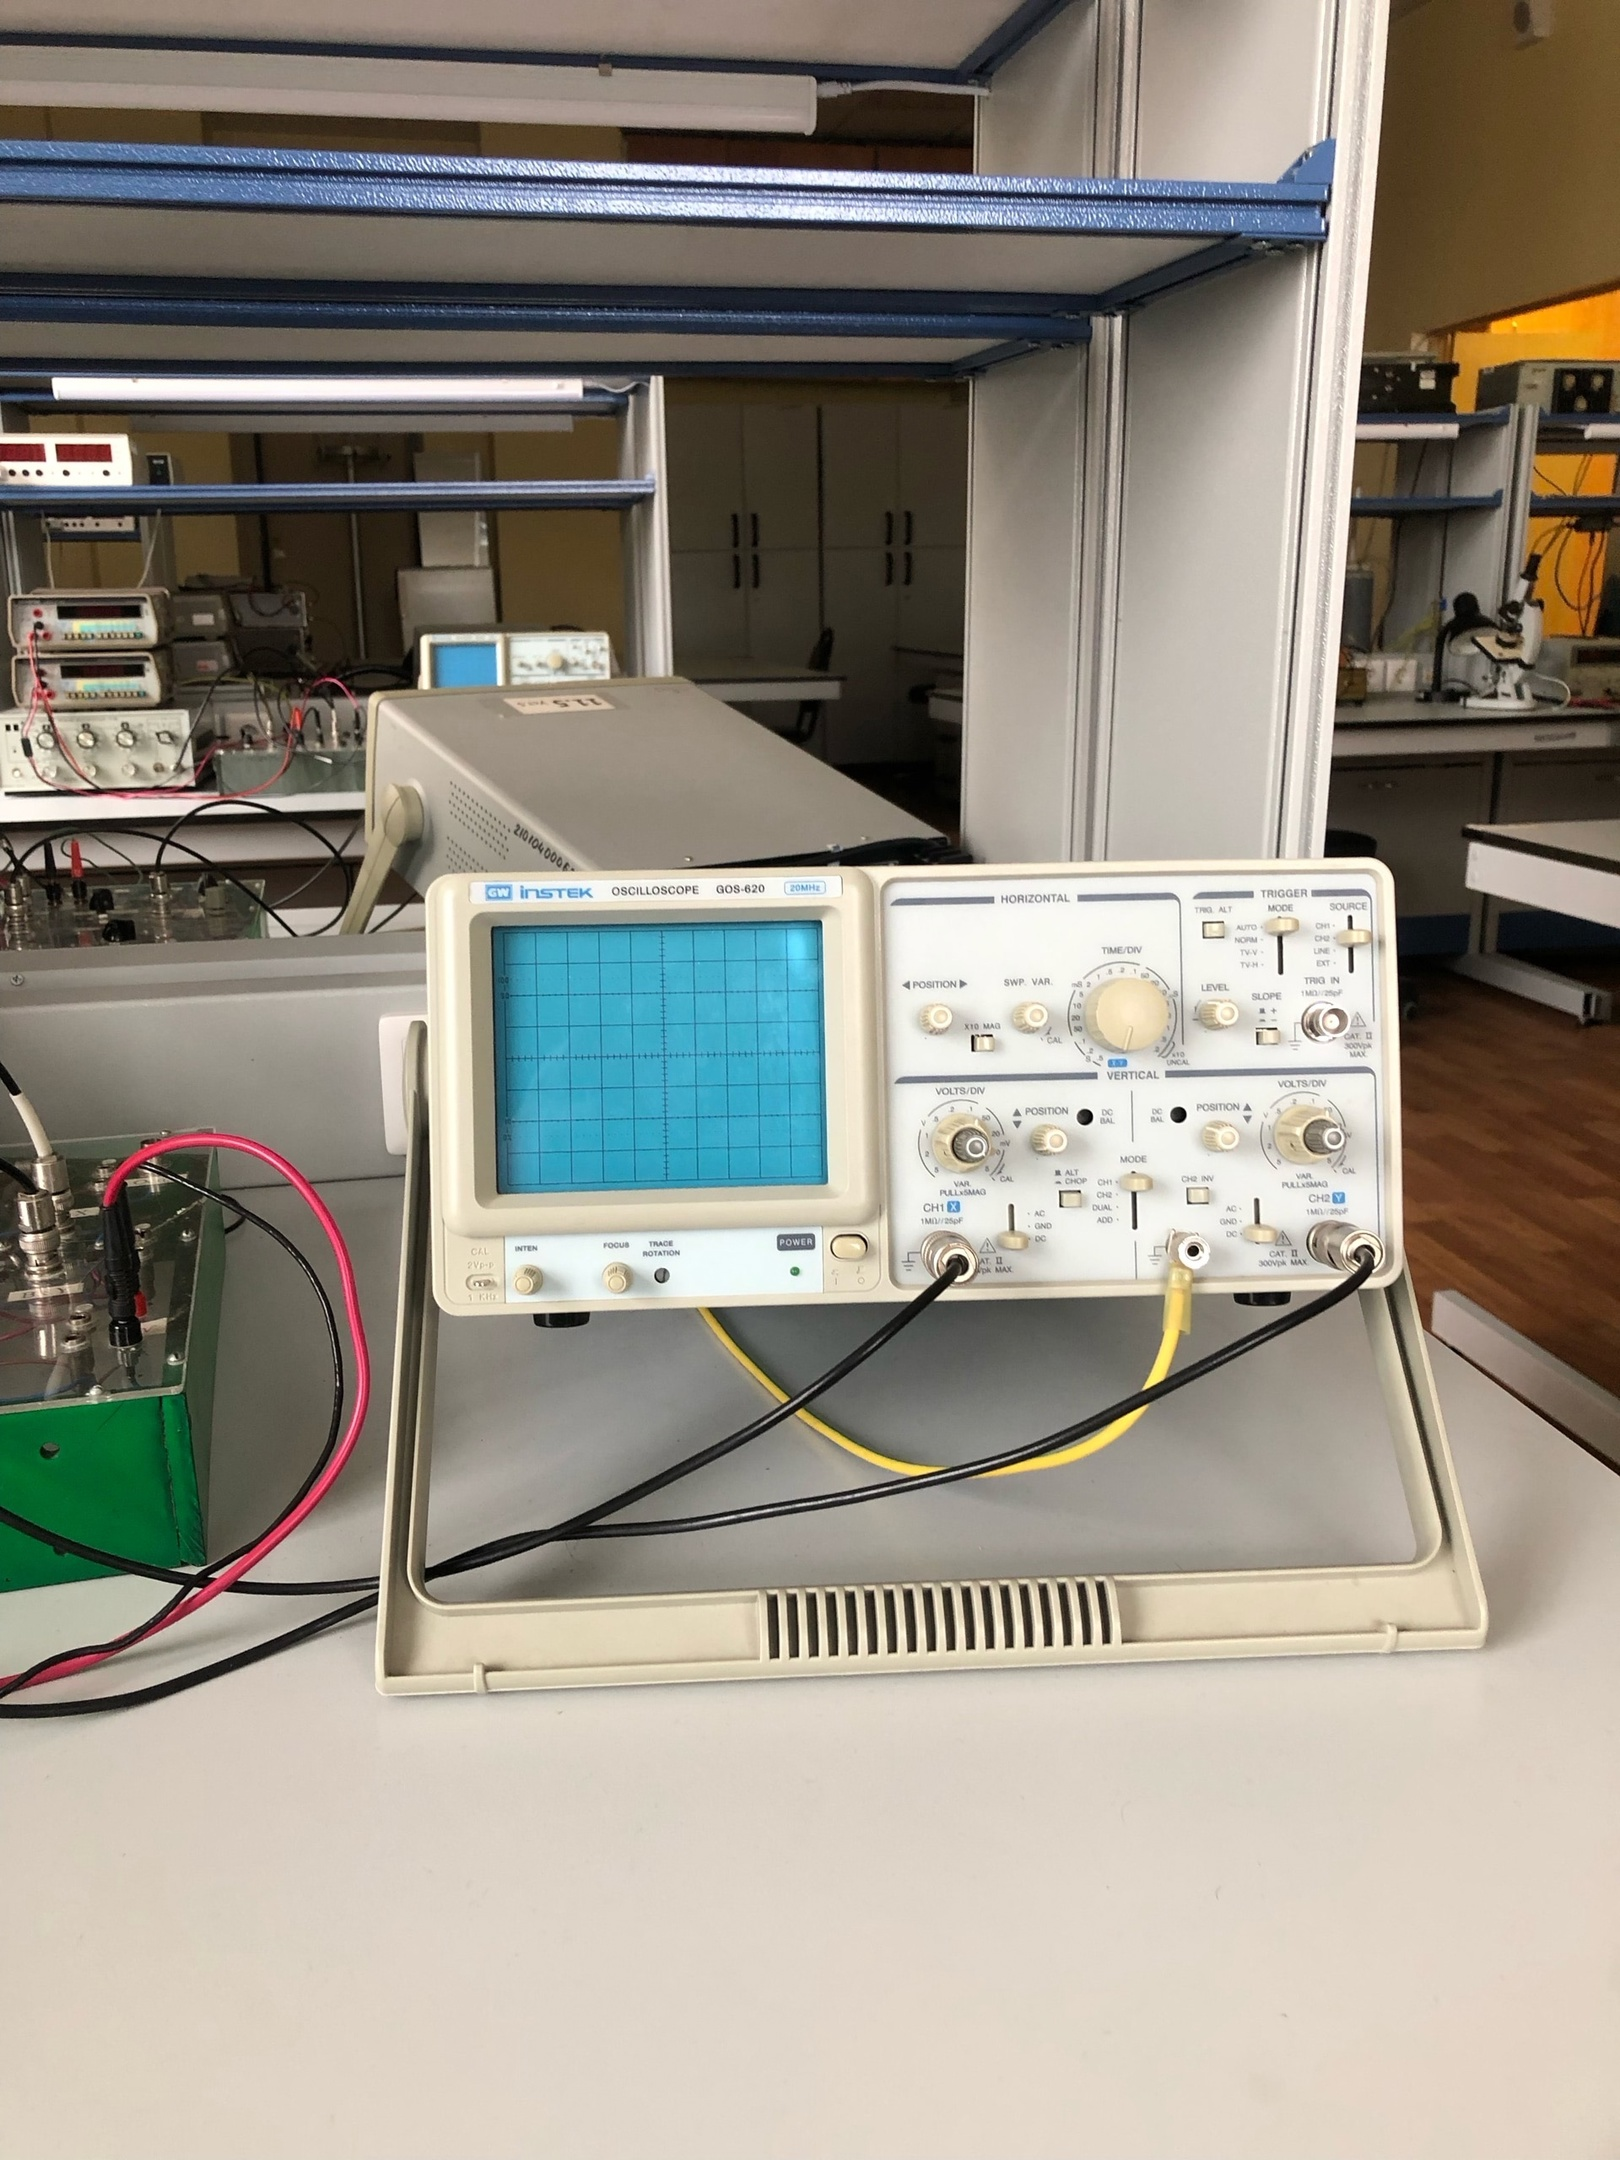
\includegraphics[width=0.3\textwidth]{3.jpg}
    \caption{Осциллограф}
    \label{pic3}
\end{figure} 

\begin{figure}[H]
    \centering	
    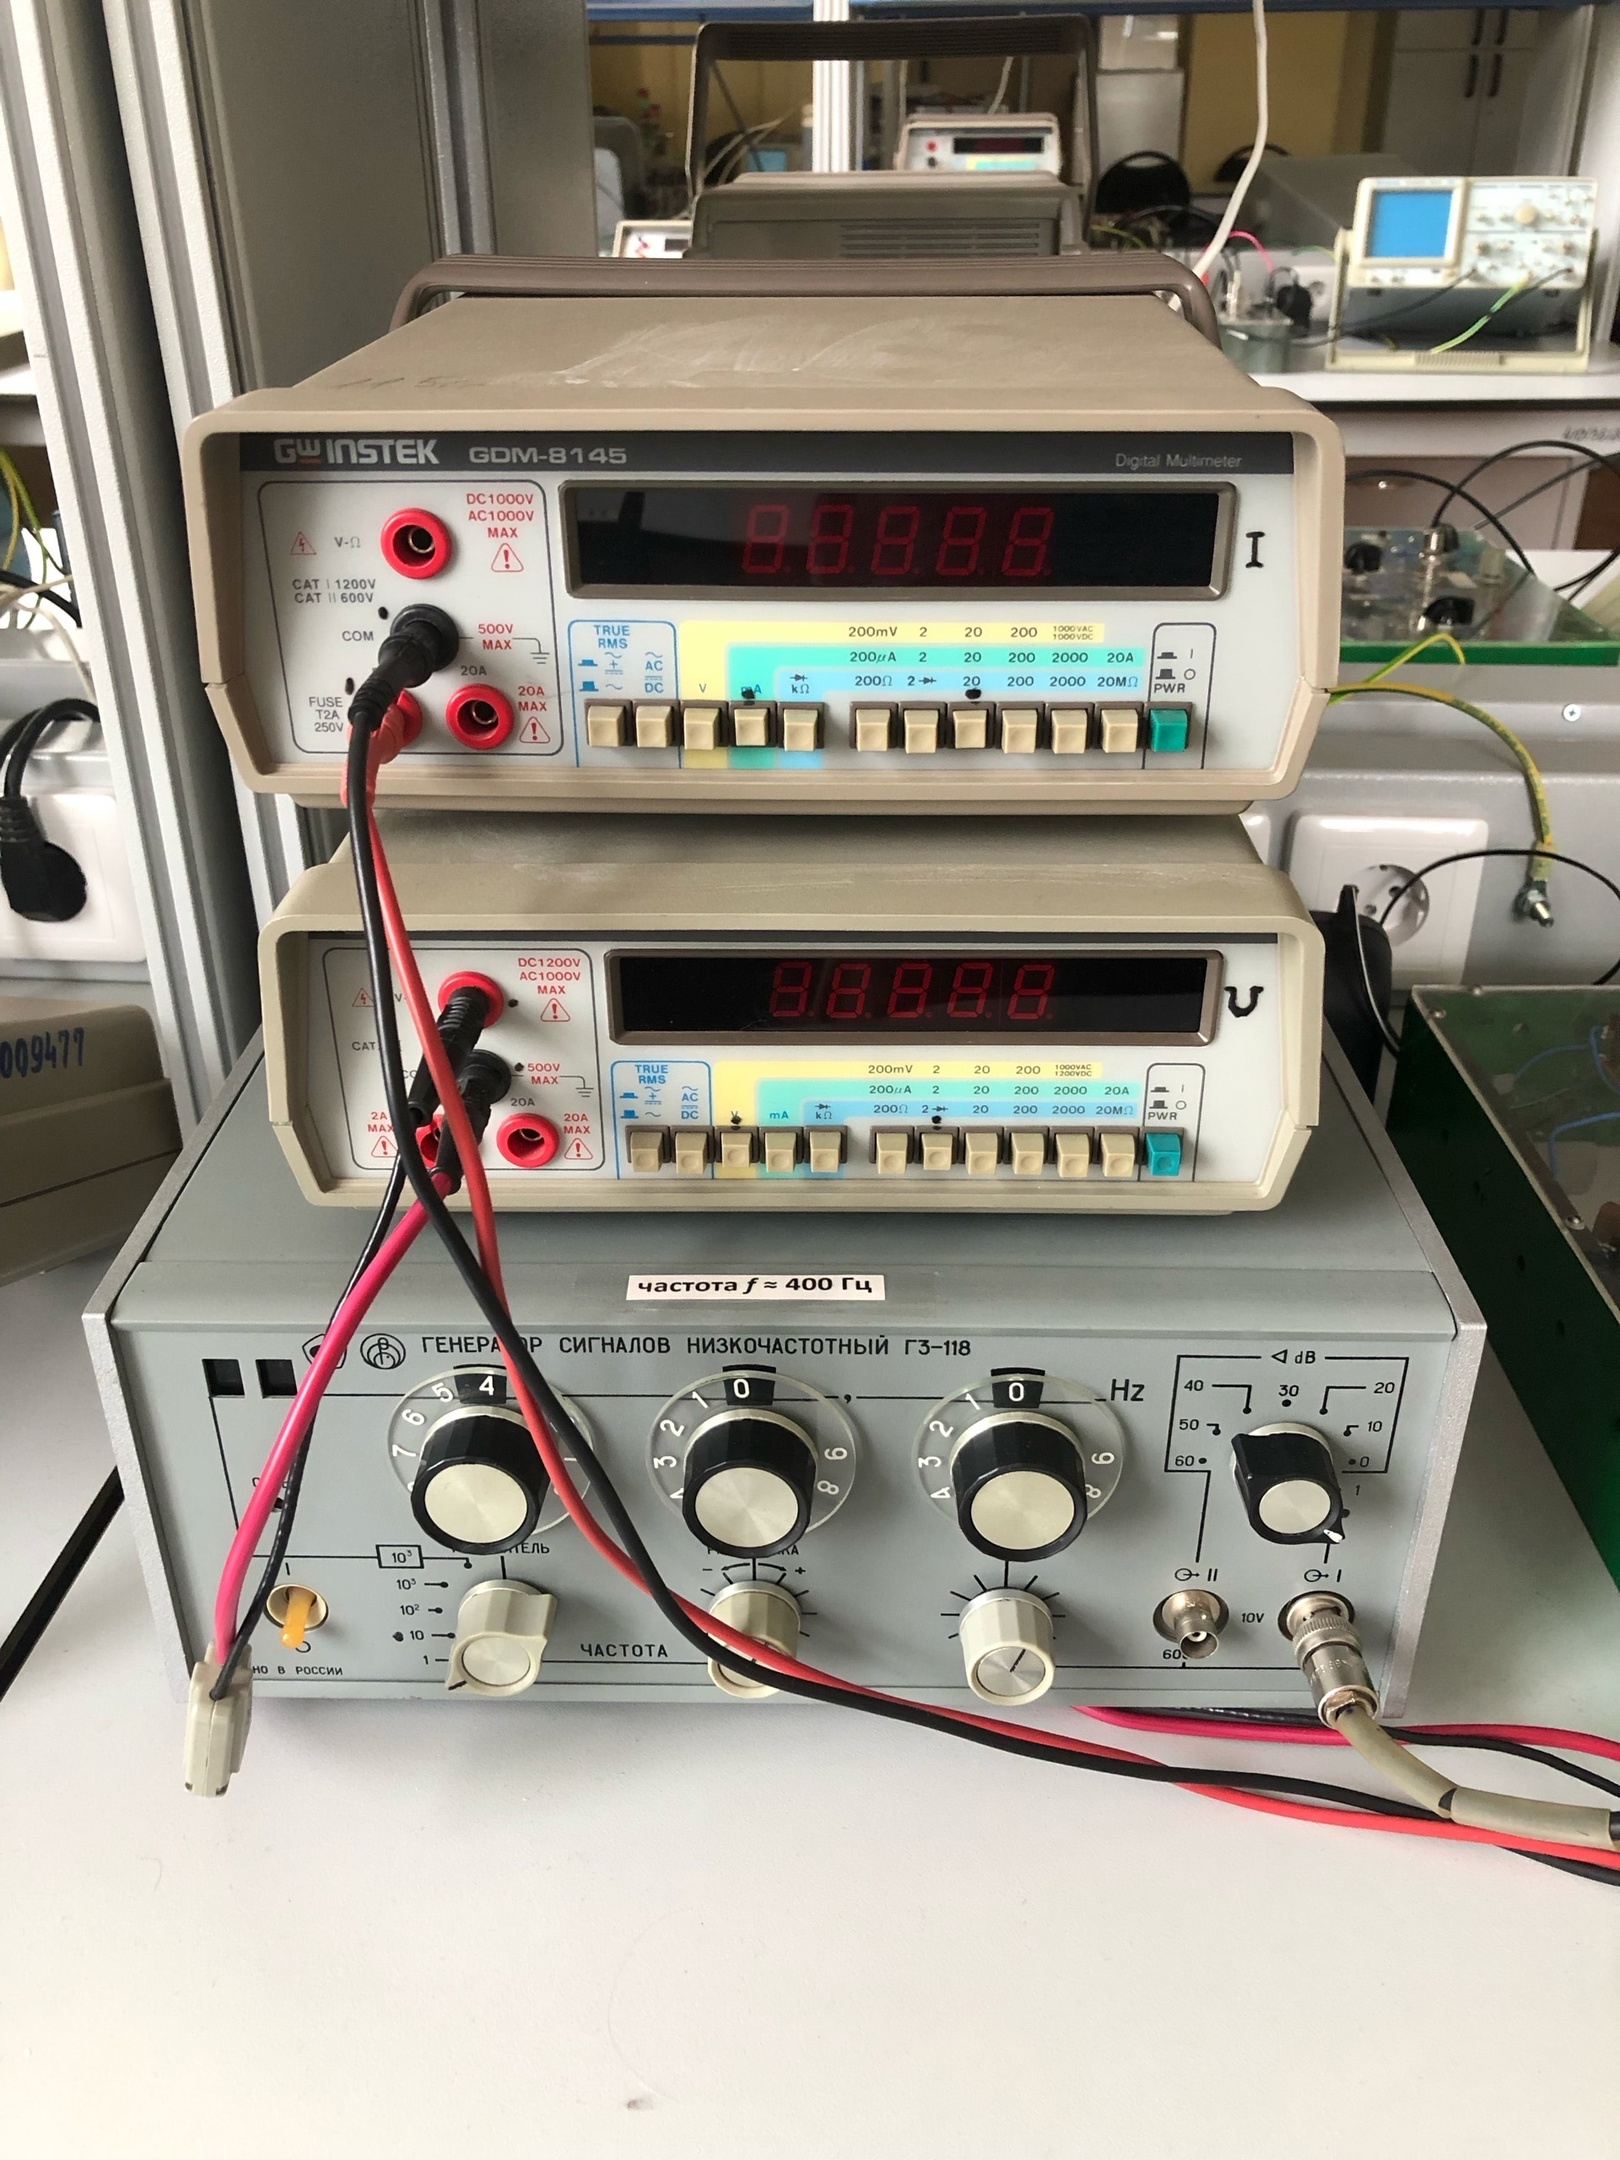
\includegraphics[width=0.3\textwidth]{2.jpg}
    \caption{Вольтметр и амперметр}
    \label{pic2}
\end{figure}

\begin{figure}[H]
    \centering	
    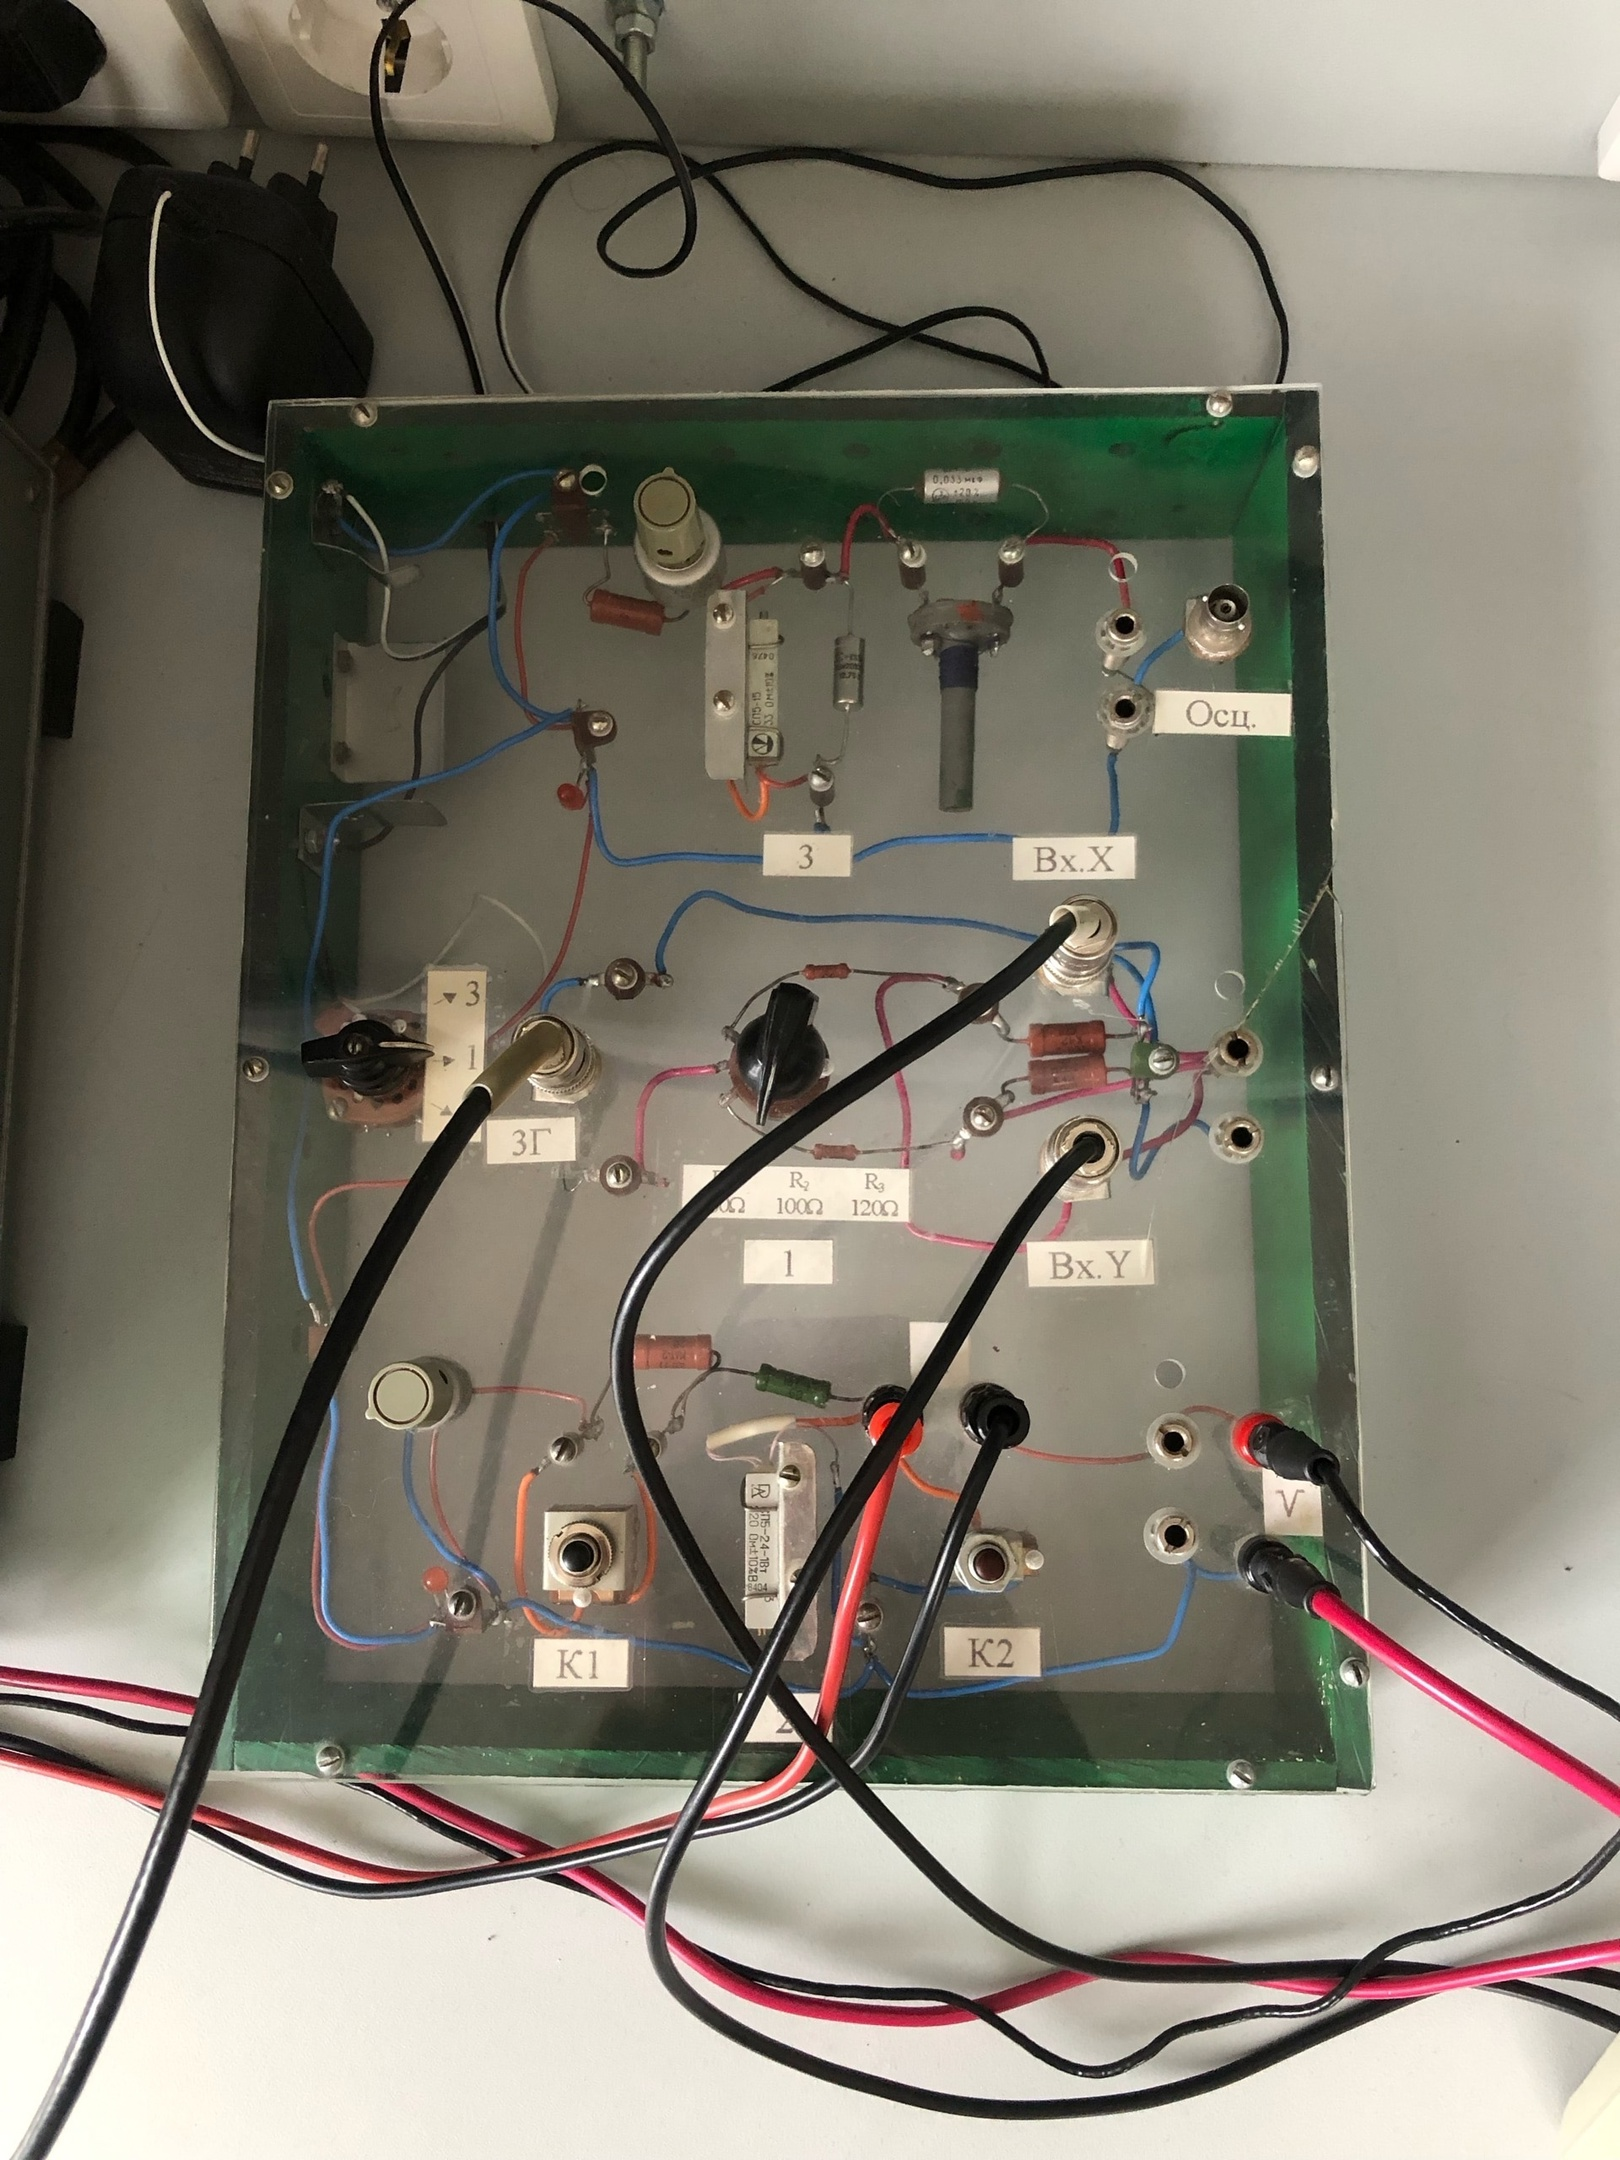
\includegraphics[width=0.3\textwidth]{1.jpg}
    \caption{Функциональная часть установки}
    \label{pic1}
\end{figure}

\section*{4. Результаты эксперимента и обработка данных}
\subsection*{4.1. Изучение ВАХ туннельного диода с помощью осциллографа}

Схема установки представлена на рисунке \ref{pic:scheme_oscil}. На вход $ Y $ осциллографа подается напряжение, пропорциональное току через диод, а на вход $ X $ --- падение напряжения на диоде.
	
\begin{figure}[H]
    \centering	
    \includegraphics[width=0.5\textwidth]{scheme_oscil.png}
    \caption{Схема наблюдения вольт-амперной характеристики туннельного диода с помощью осциллографа}
    \label{pic:scheme_oscil}
\end{figure}
	
Ток $I$ через диод зависит от напряжения $U$ на нем по следующей формуле: 
	
\[ I = U \frac{R_1 + 2(R_2 + R_3)}{(R_1 + 2R_2) \cdot R_3} \]
	
Здесь $R_1$, $R_2$, $R_3$ --- сопротивления соответствующих резисторов моста со схемы на рисунке \ref{pic:scheme_oscil}. 
	
Полученная осциллограмма для туннельного диода приведена на рисунке \ref{pic:tunnel_oscil}. 
	
\begin{figure}[H]
    \centering	
    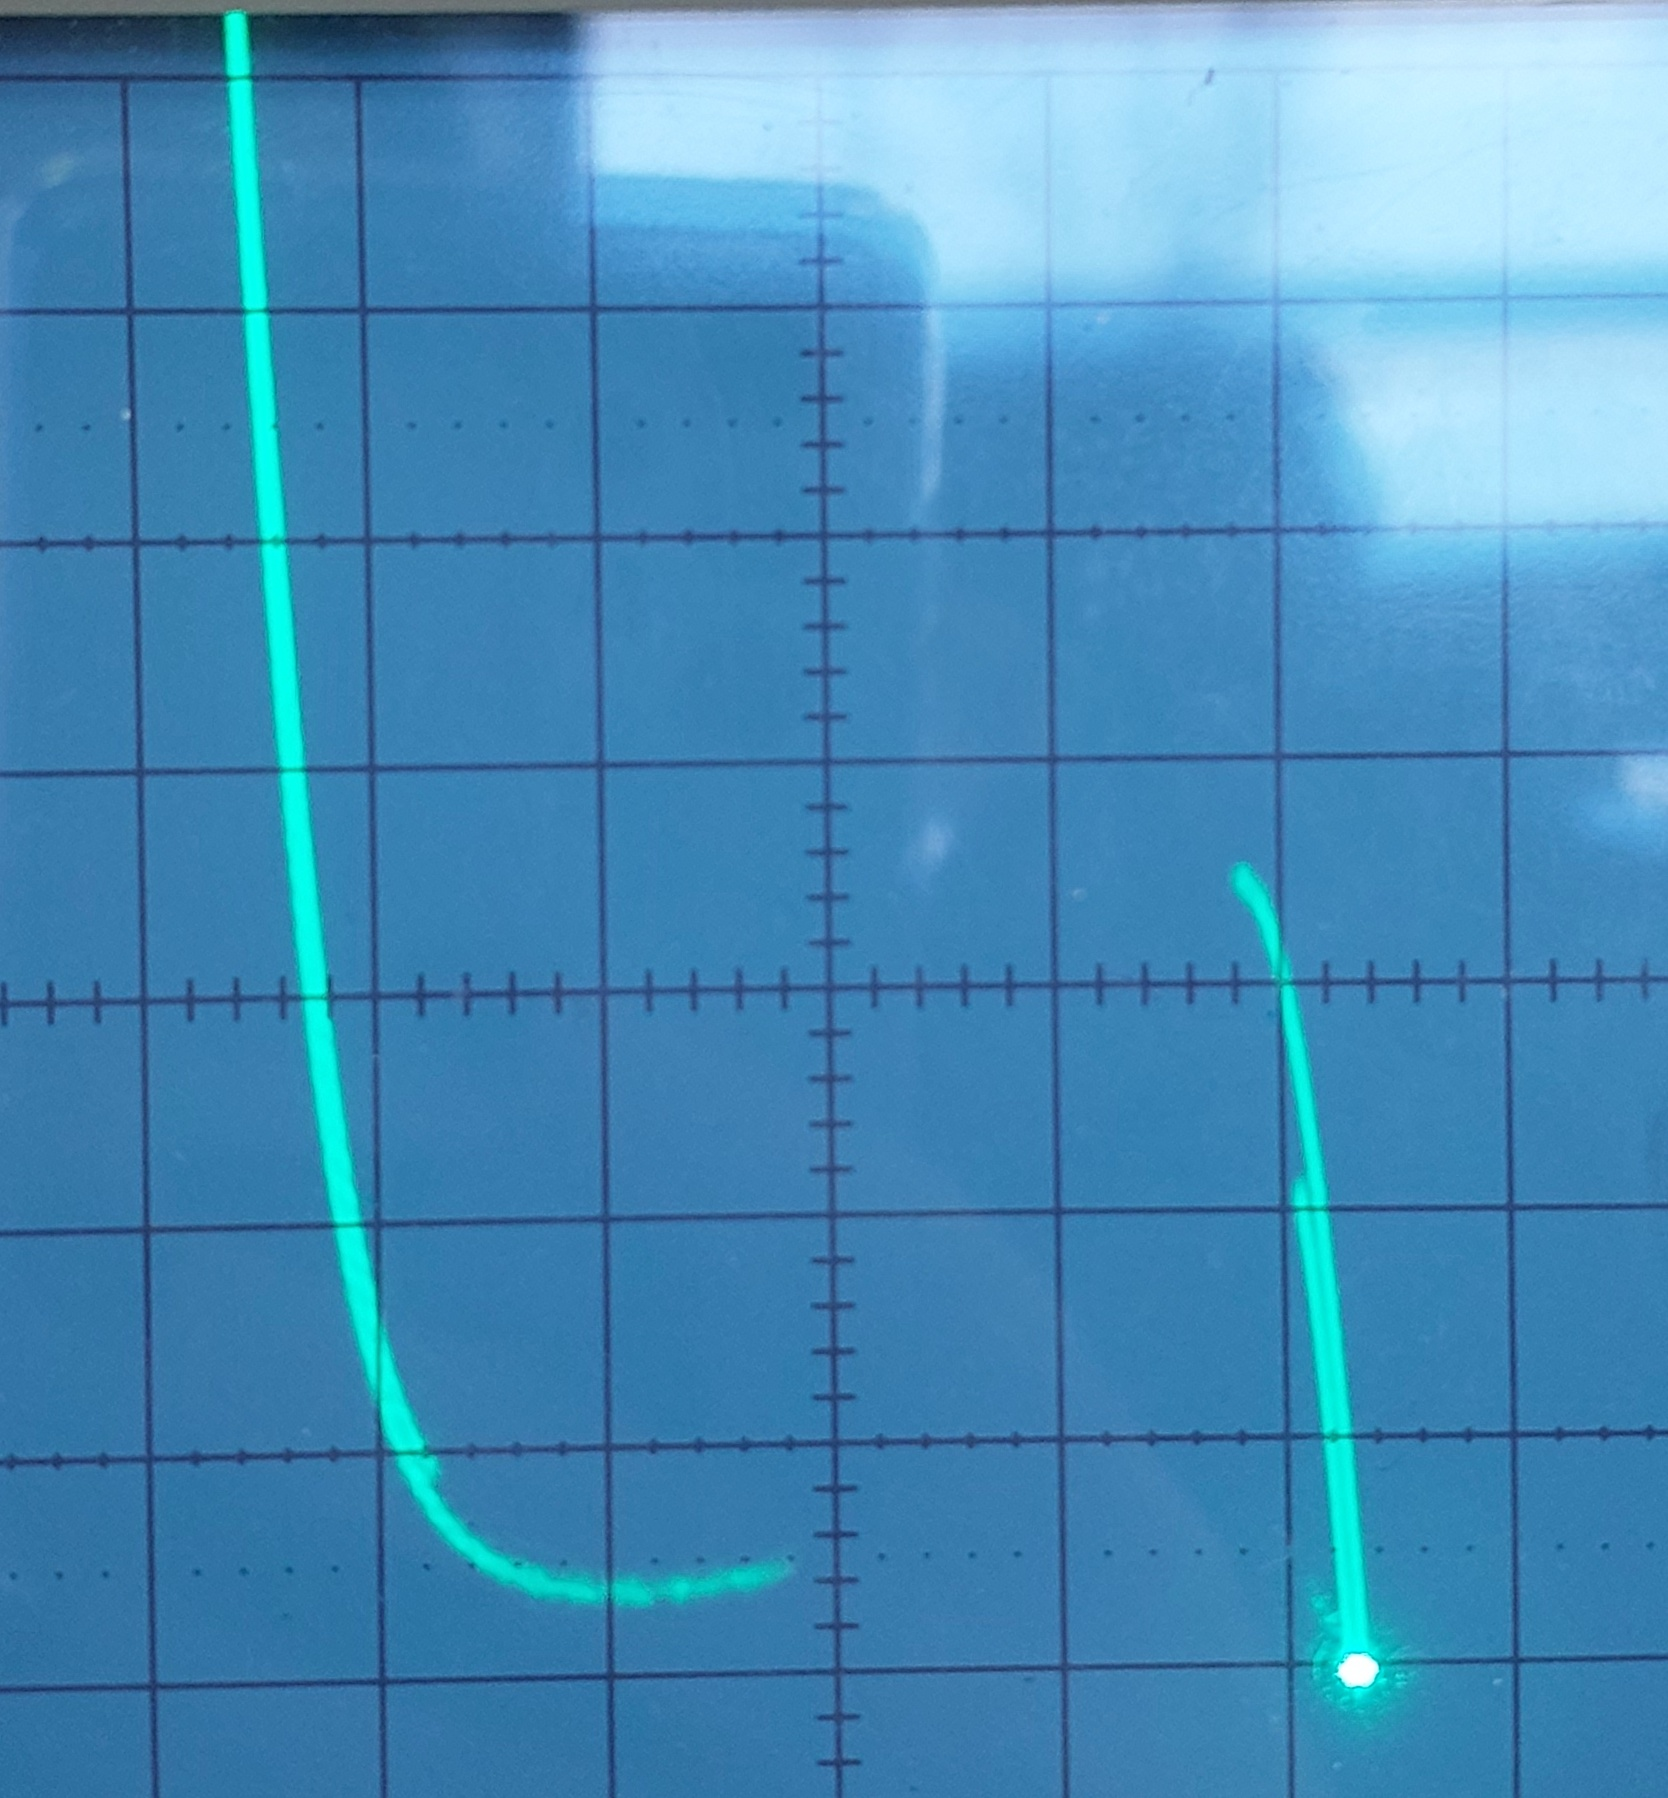
\includegraphics[width=0.3\textwidth]{oscill.jpg}
    \caption{Вольт-амперная характеристика туннельного полупроводникового диода на экране осциллографа}
    \label{pic:tunnel_oscil}
\end{figure}
	
По осциллограмме для туннельного диода оценим искомые величины напряжений (начало вольт-амперной характеристики соответствует нулевому напряжению): 
	
\[ U_p \approx 0.05 \pm  0.01 \text{ В} \]
\[ U_v \approx  0.33 \pm 0.01 \text{ В} \]
\[ U_f \approx  0.455 \pm 0.01 \text{ В} \]	

\subsection*{Получение статической характеристики туннельного диода}

Схема, используемая для получения статической характеристики диода, приведена на рисунке \ref{pic:scheme}. Ток измеряется миллиамперметром, включенным последовательно с диодом, а напряжение на диоде --- цифровым вольтметром.

\begin{figure}[H]
    \centering	
    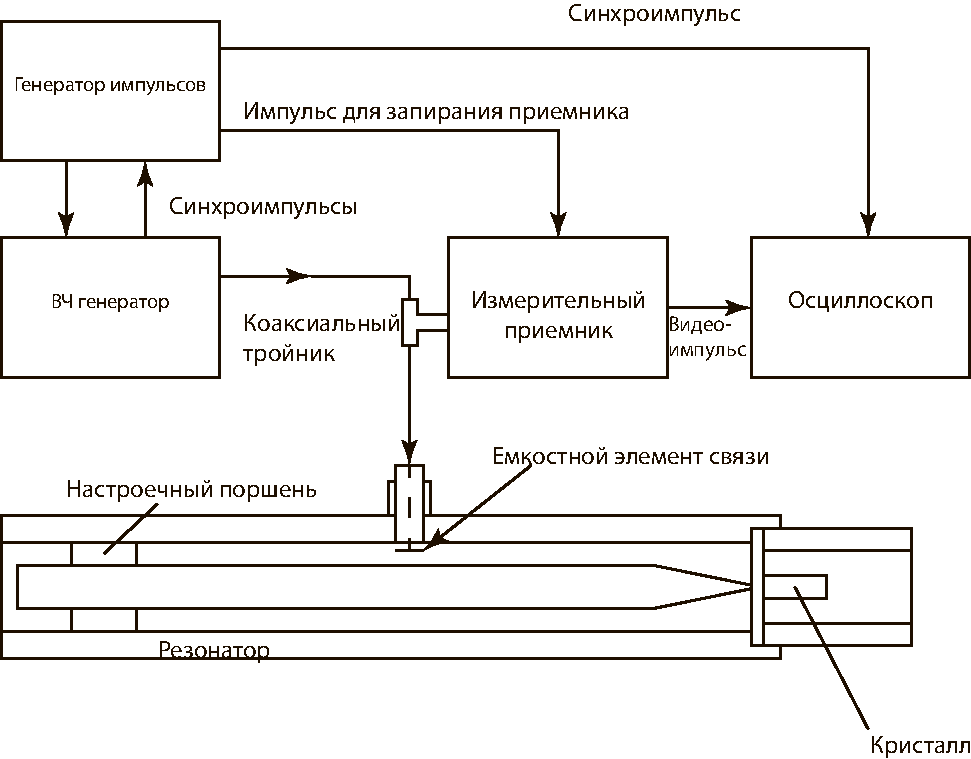
\includegraphics[width=0.5\textwidth]{scheme.png}
    \caption{Схема измерения параметров туннельного диода}
    \label{pic:scheme}
\end{figure}

Плавно меняя сопротивление резистора $ R $ и тем самым повышая напряжение на диоде, получим вольт-амперную характеристику туннельного диода $I(U)$. Погрешность величин напряжения $U$ и тока $I$ оценим двумя единицами последнего разряда. Построим график зависимости $I(U)$. Он изображен на рисунке \ref{graf}. 

\begin{figure}[H]
    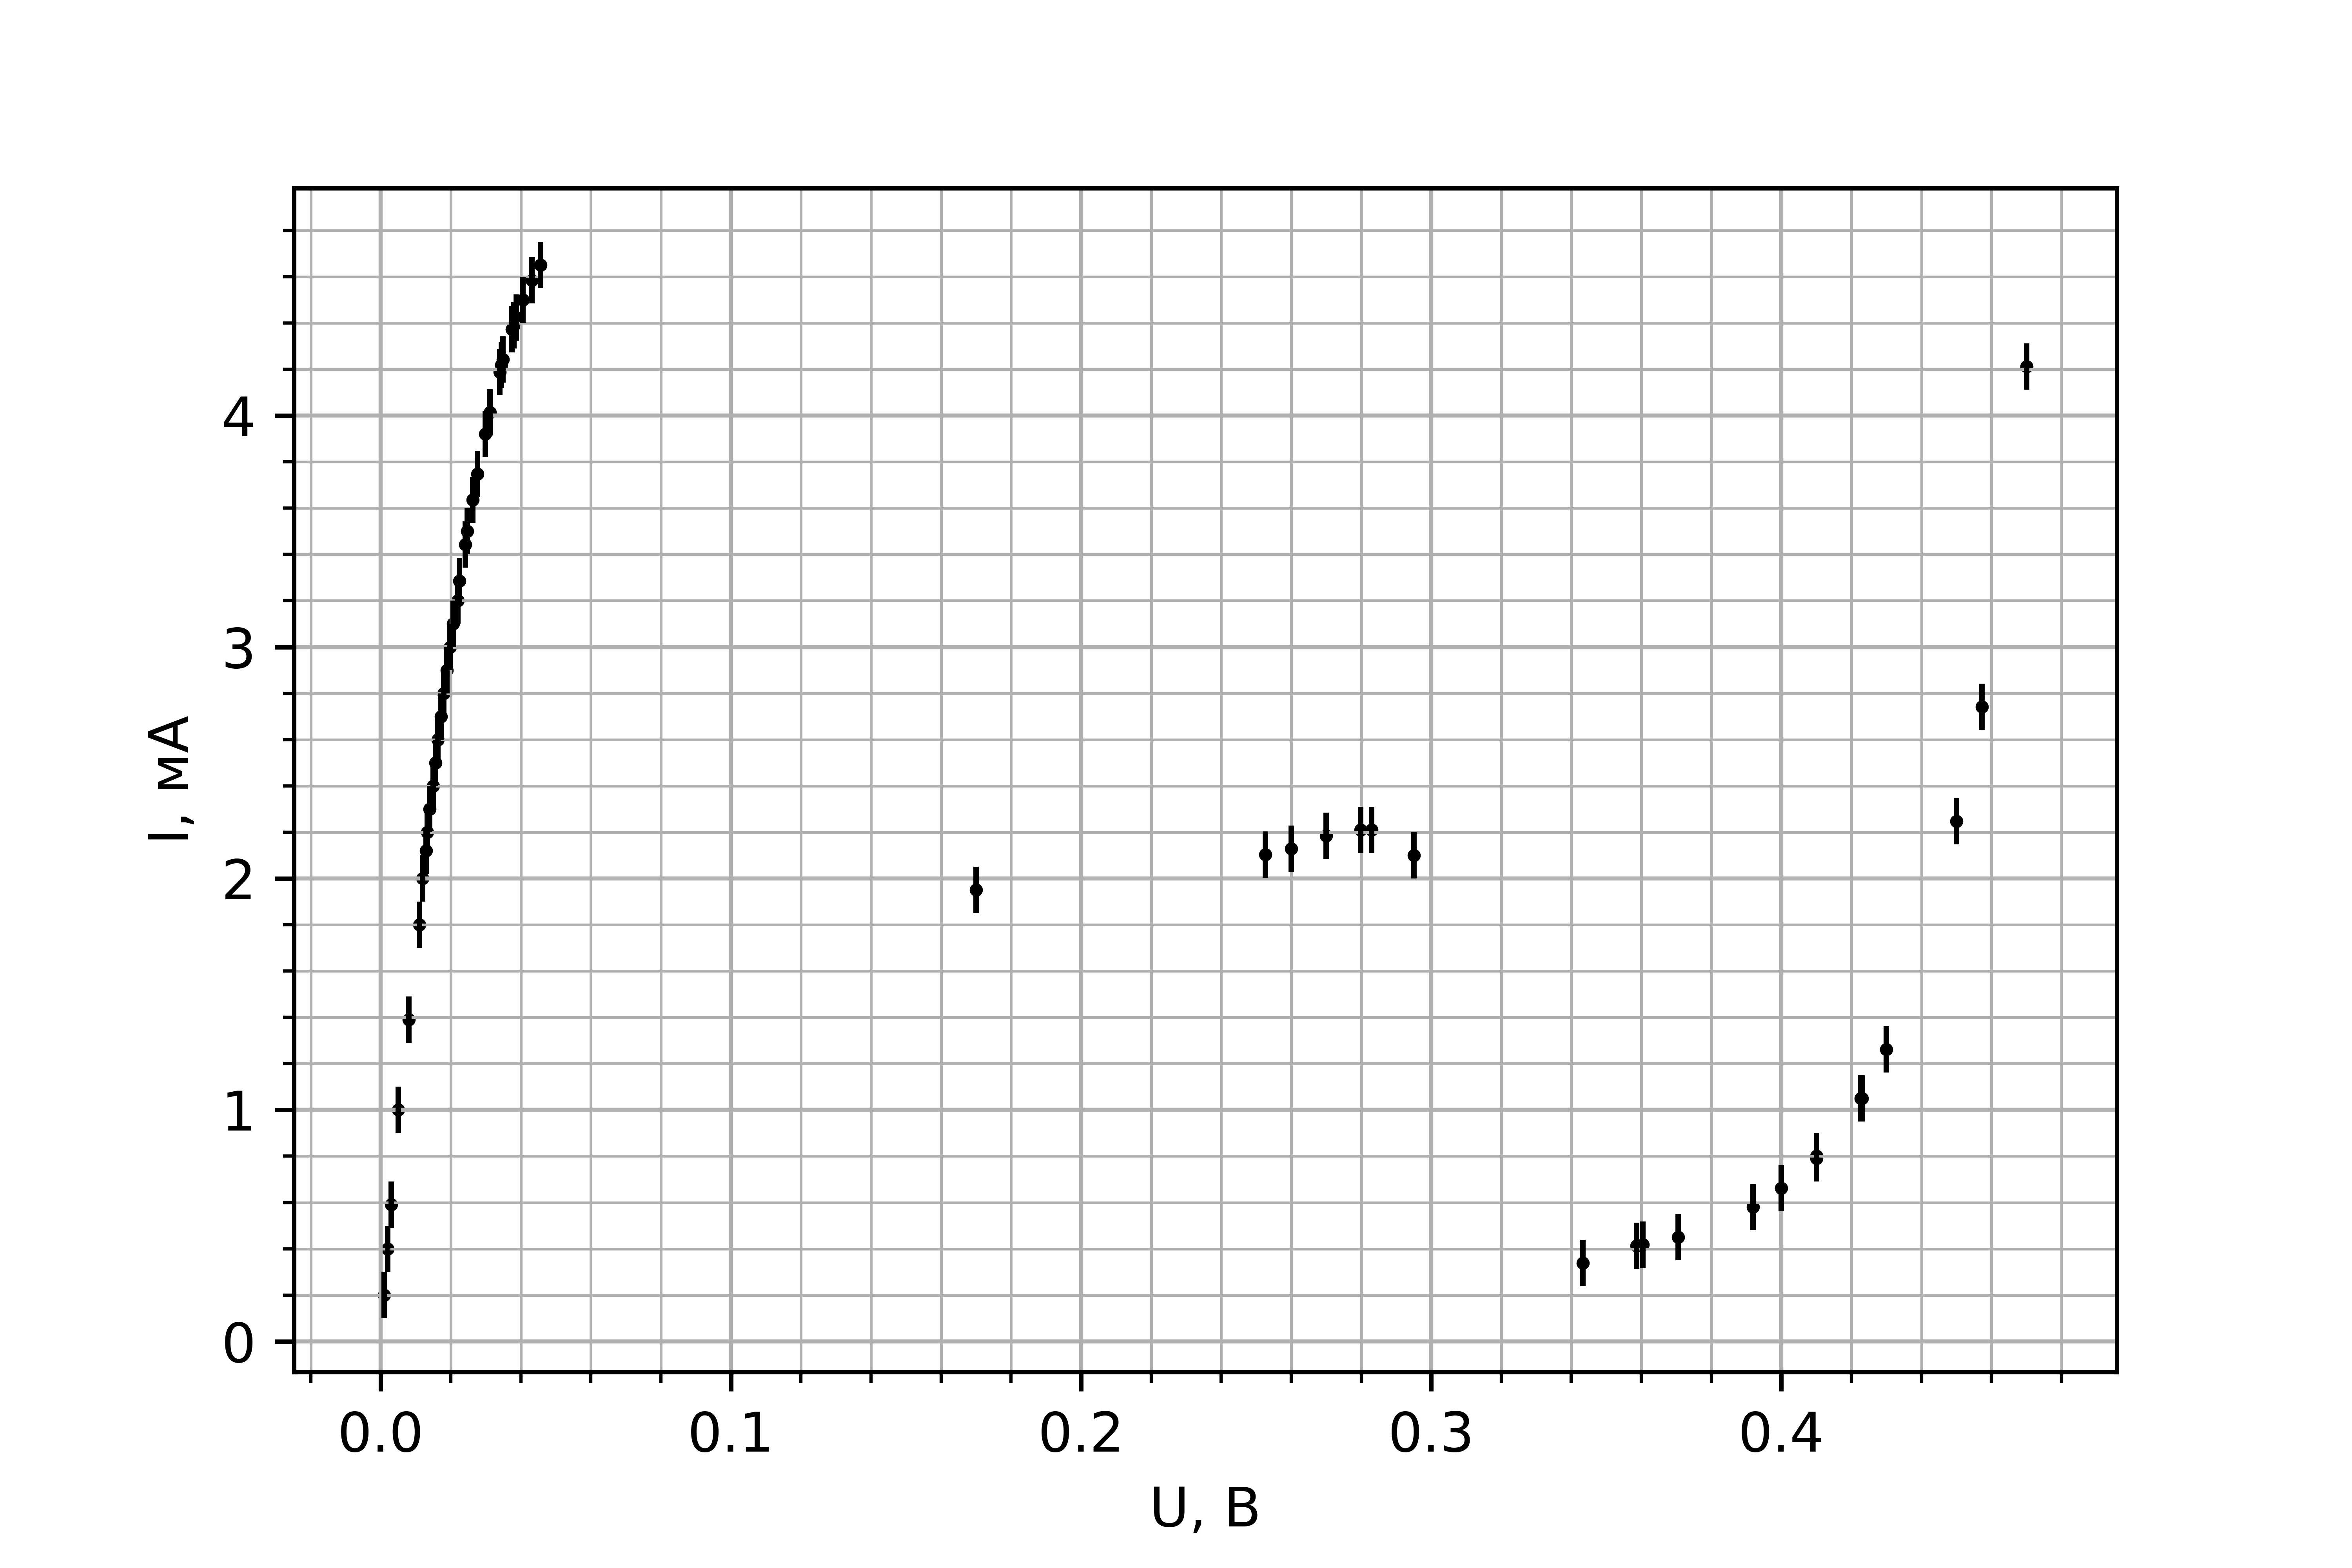
\includegraphics[scale=0.8]{I(U).png}
    \caption{Измерение вольт-амперной характеристики $I(U)$ туннельного диода}
    \label{graf}
\end{figure}

По графику определим искомые значения токов и напряжений:
	
\begin{itemize}
    \centering
    \item $ U_p = 0.04 \pm 0.02 $ В, $ I_p = 4.63 \pm 0.02 $ мА
    \item $ U_v = 0.32 \pm 0.02 $ В, $ I_v = 3.57 \pm 0.02 $ мА
    \item $ U_f = 0.47 \pm 0.02 $ В
\end{itemize} 

Примем $E_v = 0$. Тогда из выражения для $U_v \approx \frac{2\mu}{e}$ можно найти энергию Ферми $\mu_n \approx \mu_p$:

\[ \mu_n \approx \mu_p \approx eU_v/2 \approx 0.16 \text{ эВ} \]

Из выражения для напряжения $U_p \approx (\mu_n - E_\text{n max})/e$ получим энергию, соответствующую максимальной плотности распределения электронов $E_\text{n max}$:

\[ E_\text{n max} = \mu_n - eU_p \approx 0.12 \text{ эВ} \] 

\section*{5. Вывод}

В работе исследован принцип действия туннельного диода, а также получена вольт-амперная характеристика на осциллографе, затем измерена непосредственно, снимая зависимость тока от напряжения. По результатам измерений были получены параметры диода, которые в пределах погрешности совпадают с грубой оценкой, полученной благодаря наблюдению на осциллографе.

\newpage
\section*{6. Приложение}
\begin{table}[H]
\begin{tabular}{|c|c|}
\hline
$I$, мА & $U$, В   \\ \hline
0.2   & 0.001  \\ \hline
0.4   & 0.002  \\ \hline
0.59  & 0.003  \\ \hline
1     & 0.005  \\ \hline
1.39  & 0.008  \\ \hline
1.8   & 0.011  \\ \hline
2     & 0.012  \\ \hline
2.12  & 0.013  \\ \hline
2.2   & 0.0133 \\ \hline
2.3   & 0.014  \\ \hline
2.4   & 0.015  \\ \hline
2.5   & 0.0156 \\ \hline
2.6   & 0.0163 \\ \hline
2.7   & 0.0172 \\ \hline
2.8   & 0.018  \\ \hline
2.9   & 0.0189 \\ \hline
3     & 0.0198 \\ \hline
3.1   & 0.0207 \\ \hline
3.2   & 0.022  \\ \hline
3.285 & 0.0225 \\ \hline
3.443 & 0.0241 \\ \hline
3.5   & 0.0247 \\ \hline
3.636 & 0.0263 \\ \hline
3.748 & 0.0276 \\ \hline
3.921 & 0.0299 \\ \hline
4.014 & 0.0312 \\ \hline
4.188 & 00.034 \\ \hline
4.218 & 0.0345 \\ \hline
\end{tabular}
\hspace{1.5 cm}
\begin{tabular}{|c|c|}
\hline
$I$, мА & $U$, В   \\ \hline
4.242 & 0.0349 \\ \hline
4.372 & 0.0375 \\ \hline
4.389 & 0.038  \\ \hline
4.424 & 0.0387 \\ \hline
4.5   & 0.0406 \\ \hline
4.585 & 0.0432 \\ \hline
4.65  & 0.0456 \\ \hline
2.103 & 0.2526 \\ \hline
2.128 & 0.26   \\ \hline
2.185 & 0.27   \\ \hline
2.210 & 0.2798 \\ \hline
2.21  & 0.283  \\ \hline
2.1   & 0.295  \\ \hline
0.8   & 0.41   \\ \hline
1.05  & 0.423  \\ \hline
1.95  & 0.17   \\ \hline
0.338 & 0.3433 \\ \hline
0.413 & 0.3586 \\ \hline
0.418 & 0.3604 \\ \hline
0.45  & 0.3705 \\ \hline
0.58  & 0.3919 \\ \hline
0.662 & 0.4    \\ \hline
0.79  & 0.41   \\ \hline
1.049 & 0.4227 \\ \hline
1.262 & 0.43   \\ \hline
2.247 & 0.45   \\ \hline
2.742 & 0.4573 \\ \hline
4.212 & 0.47   \\ \hline
\end{tabular}
\caption{Результаты измерений ВАХ туннельного диода}
\end{table}


\end{document}
